%%%%%%%%%%%%%%%%%%%%%%%%%%%%%%%%%%%%%%%%%%%%%%%%%%%%%%%%%%%%%%%%%%%%%%%%%%%%%%%%
%2345678901234567890123456789012345678901234567890123456789012345678901234567890
%        1         2         3         4         5         6         7         8
\documentclass[a4paper,11pt]{article}
%\documentclass[letterpaper, 10 pt, conference]{ieeeconf}  % Comment this line out if you need a4paper
%\documentclass[a4paper, 10pt, conference]{ieeeconf}      % Use this line for a4 paper
%\IEEEoverridecommandlockouts                              % This command is only needed if 
                                                          % you want to use the \thanks command
%\overrideIEEEmargins                                      % Needed to meet printer requirements.

% See the \addtolength command later in the file to balance the column lengths
% on the last page of the document

% The following packages can be found on http:\\www.ctan.org
\usepackage{graphics} % for pdf, bitmapped graphics files
\usepackage{epsfig} % for postscript graphics files
\usepackage{mathptmx} % assumes new font selection scheme installed
\usepackage{times} % assumes new font selection scheme installed
\usepackage{amsmath} % assumes amsmath package installed
\usepackage{amssymb}  % assumes amsmath package installed
\usepackage{booktabs}  % assumes amsmath package installed
	
\title{\LARGE \bf
Controlling a cadaveric hand and identifying realistic parameters with a simulated spinal cord.
}

\author{Valero-Cuevas FJ, Jalaleddini K, Chakravarthi S, Poblete K, and Cohn BA$^{1}$ % <-this % stops a space
\thanks{*This work was supported by NIH NIAMS R01AR050520 and R01AR052345 grants, and SNF Project 200021-150055-1 [FcoTodo Check].
}% <-this % stops a space
\thanks{$^{1}$Departments of Biomedical Engineering and Computer Science at the University of Southern California Viterbi School of Engineering, Los Angeles, CA 90089, USA
        {\tt\small brianaco@usc.edu}}%
}
\begin{document}
\maketitle
%\thispagestyle{empty}
%\pagestyle{empty}
%%%%%%%%%%%%%%%%%%%%%%%%%%%%%%%%%%%%%%%%%%%%%%%%%%%%%%%%%%%%%%%%%%%%%%%%%%%%%%%%
\begin{abstract}
[briantodo abstract]
\end{abstract}
%%%%%%%%%%%%%%%%%%%%%%%%%%%%%%%%%%%%%%%%%%%%%%%%%%%%%%%%%%%%%%%%%%%%%%%%%%%%%%%%
\section{INTRODUCTION}
There are many papers out there.

\section{METHODS}

 The system used for all experiments consists of a carefully selected set of hardware, sofware, and materials.

For our tendons, we use [@victor material] strings instead of string or wire, so they are less prone to damage from wetting in cadaveric experiments, and so the wire stress extension is minimal.

 Two identical systems were designed, one to be used primarily for cadaveric experiments (wet lab) and another for exclusively non-biological specimens (dry lab).

\\subsection{FPGA Controller implementation} % (fold)
\label{sub:fpga_controller_implementation}
An FPGA is a field-programmable gate array- a small circuit which can represent functions as circuit implementations.
We opted to use FPGA in exploring these points:
\item FPGA's run in a deterministic time, and thus their latencies are several orders of magnitude faster than even an optimized CPU implementation. We have the opportunity to set the clock timing to exactly the rate we want, while GPU procesing could become lagged.
\item With consistent clock frequency being of paramount importance, the FPGA has low-variance in delivering results, becuase it's powered by an independent hardware timer that's dedicated to the FPGA.

FPGA Card (NI PXI-7952R FlexRIO)
DAQ Card (NI PXI-625X)
Timing I/O Card (NI PXI-6602) - Receives the encoder pulses, and receives the pulses per second to 
DC Motor, Encoder, Gear Head  (Faulhaber 3883H024C+HEDS5500A12 + X074343)
PXI Chassis (NI PXI-104x )
Embedded Controller + CPU (NI PXI-8108)




We used a PXI Bus to handle the direct memory acess between the FPGA IO buffers and the DAQ (NI PXI-625X).


\begin{figure}[schematic_finger_overhead]
  \label{fig:schematic_finger_overhead}
  \centering
  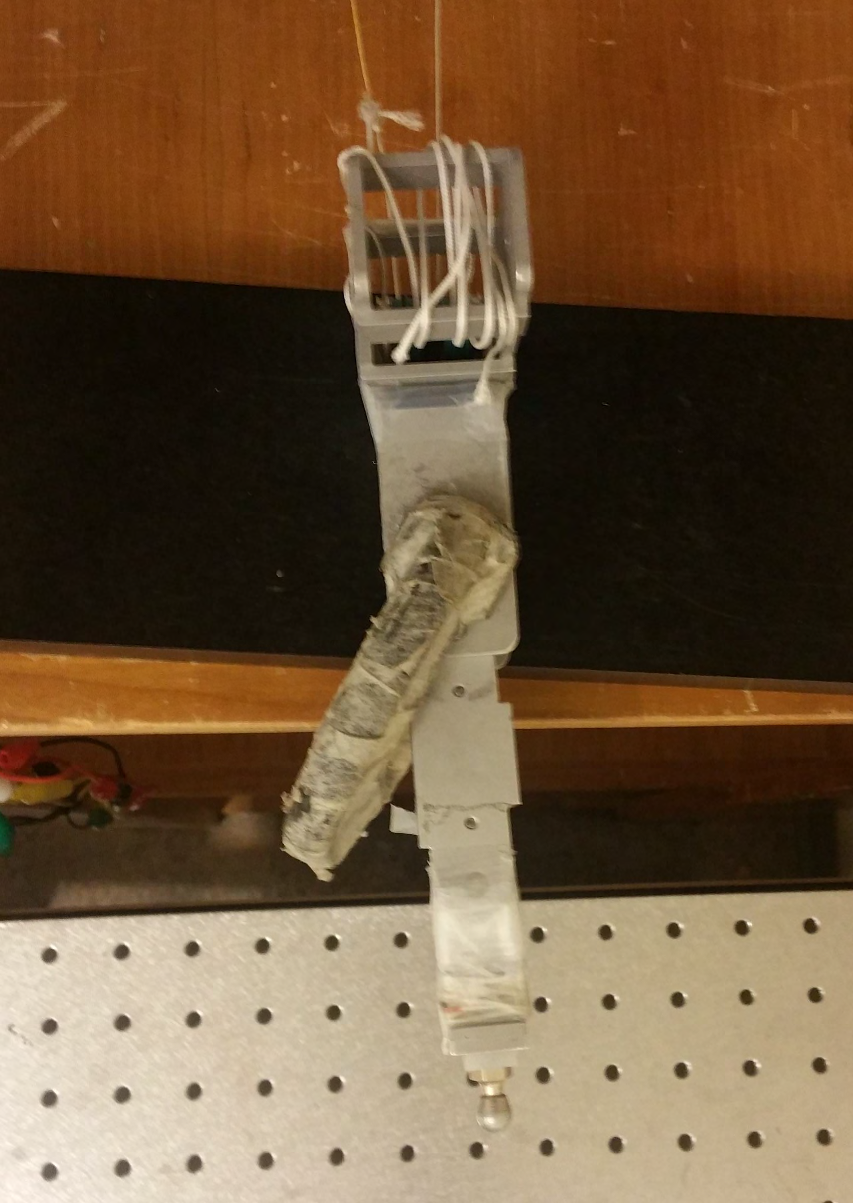
\includegraphics[width=0.5\textwidth]{figures/overhead_robotic_finger.pdf}
  \caption{Tendon driven robotic finger with one joint, 1DOF, 2 muscles}
\end{figure}

\begin{figure}[hardware_schematic]
  \label{fig:hardware_schematic}
  \centering
  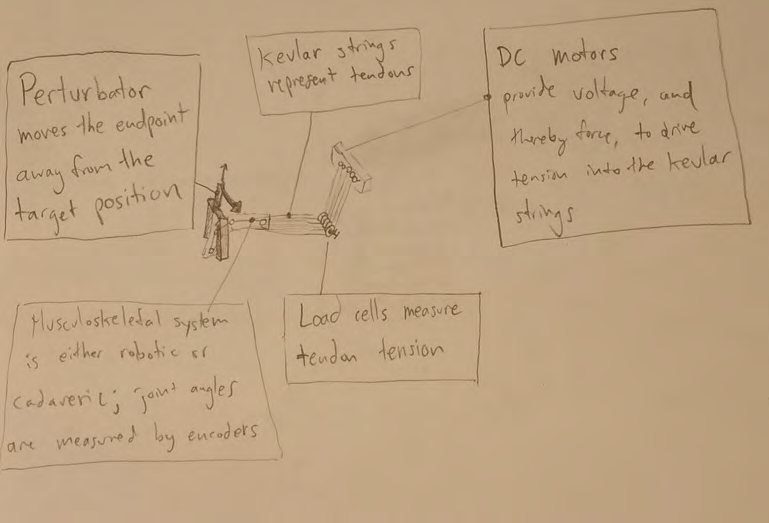
\includegraphics[width=1.0\textwidth]{figures/hardware_schematic.pdf}
  \caption{Caption one two three}
\end{figure}

\begin{figure}[fpga_schematic]
  \label{fig:fpga_schematic}
  \centering
  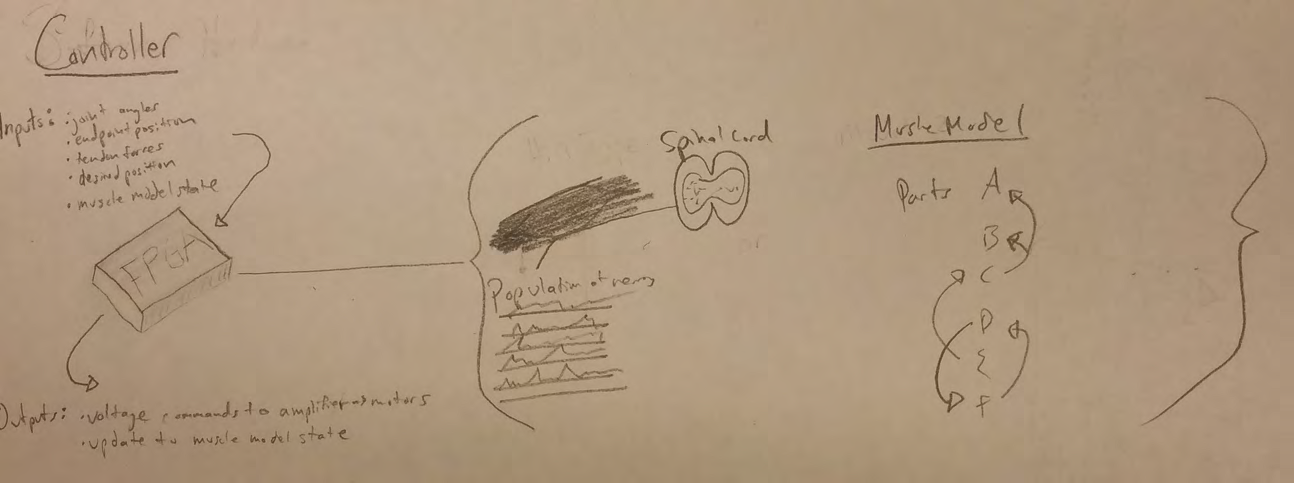
\includegraphics[width=1.0\textwidth]{figures/fpga_schematic.pdf}
  \caption{Caption one two three}
\end{figure}


\begin{figure}[loadcells_pulley]
  \label{fig:loadcells_pulley}
  \centering
  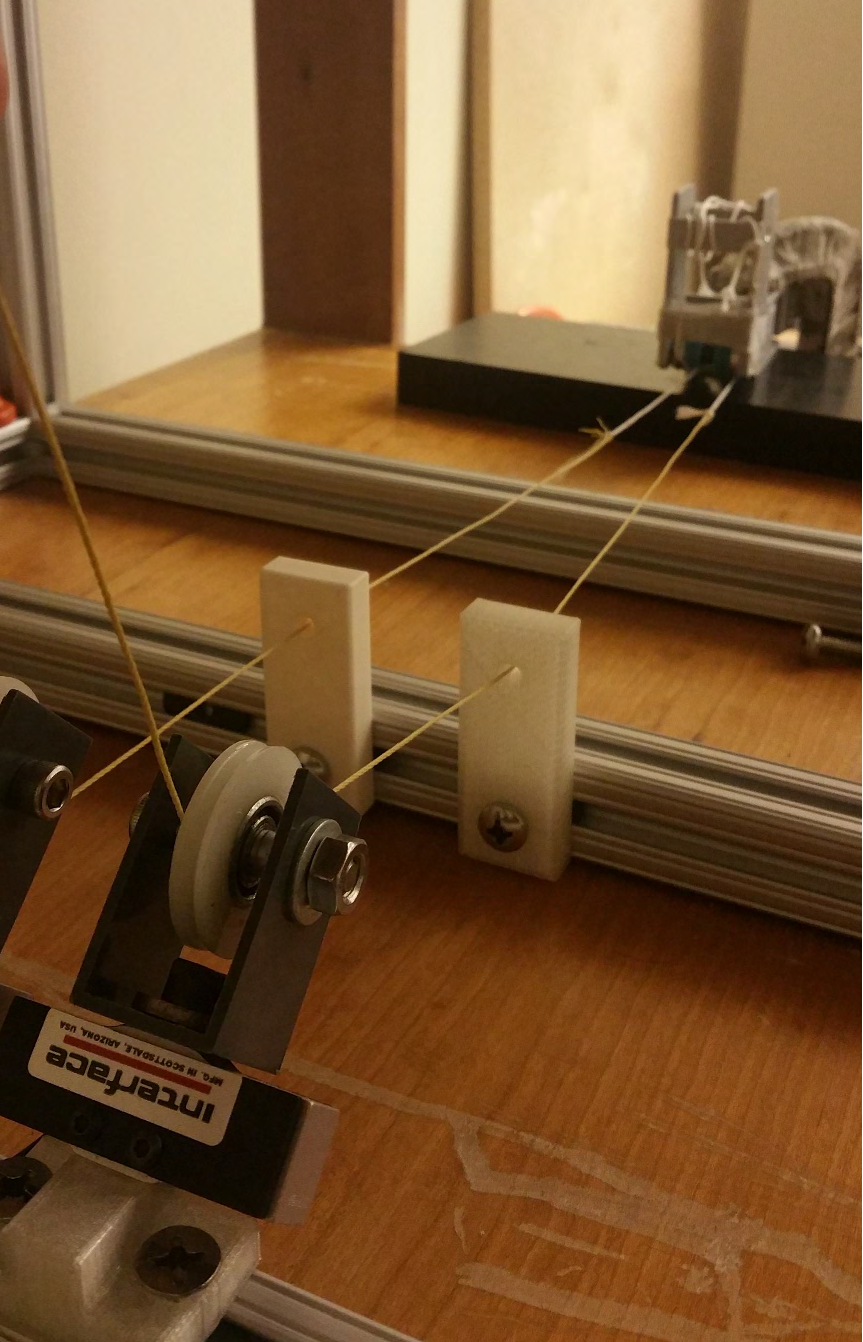
\includegraphics[width=0.5\textwidth]{figures/loadcells_pulley.pdf}
  \caption{Caption one two three}
\end{figure}
\begin{figure}[motor_closeup]
  \label{fig:motor_closeup}
  \centering
  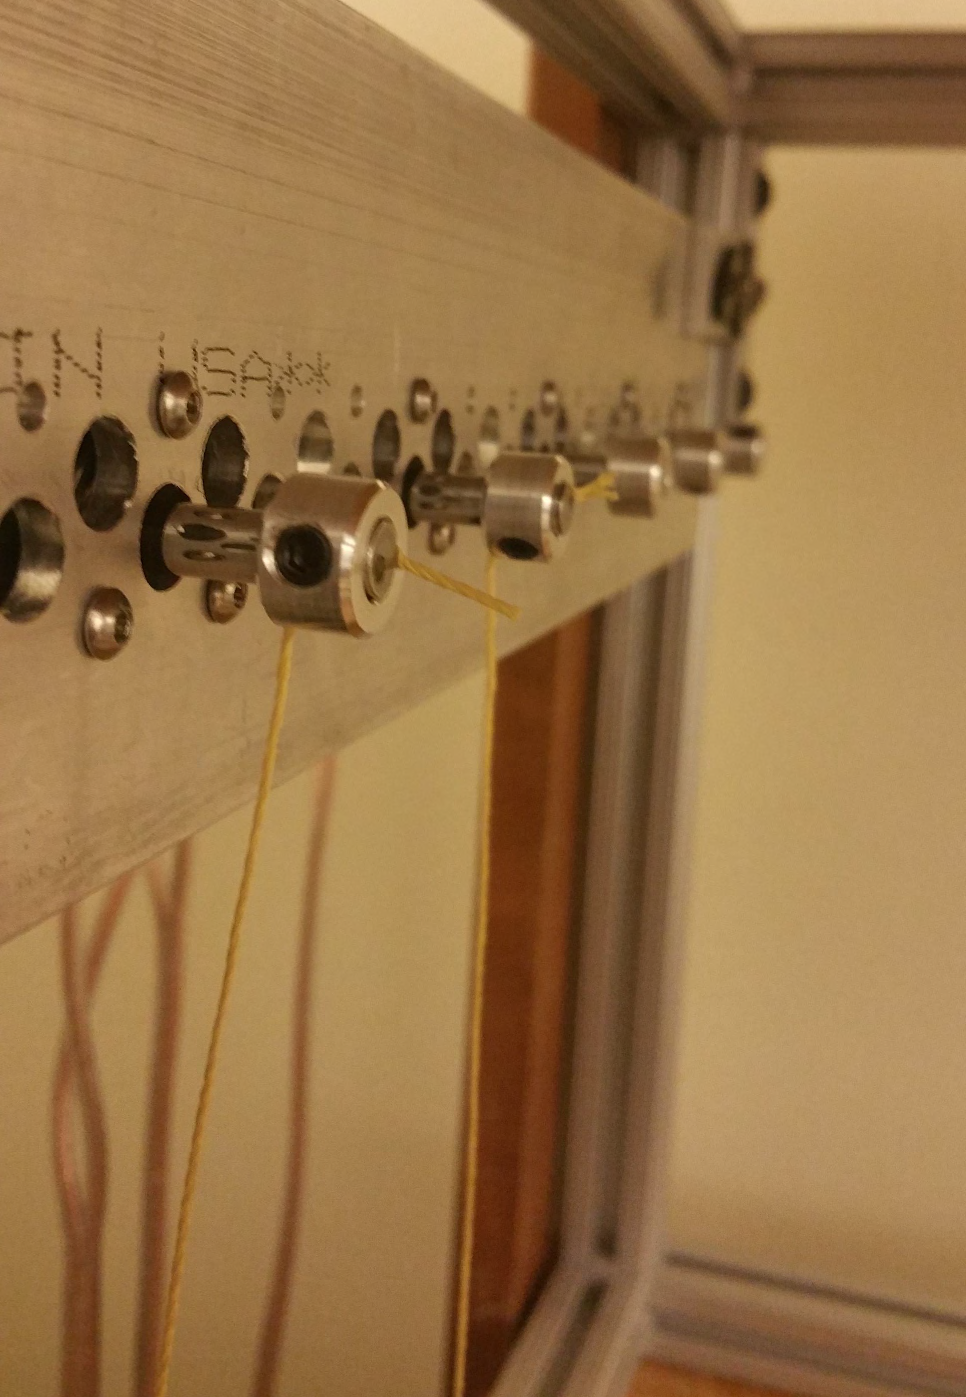
\includegraphics[width=0.5\textwidth]{figures/motor_closeup.pdf}
  \caption{Caption one two three}
\end{figure}

\section{RESULTS}
[briantodo make a few sample plots in R]
\section{DISCUSSION}

Our results provide evidence supporting the following:
\begin{itemize}
	\item{Firstthing}
	\item{Secondthing}
	\item{Thirdthing}
\end{itemize}
%%%%%%%%%%%%%%%%%%%%%%%%%%%%%%%%%%%%%%%%%%%%%%%%%%%%%%%%%%%%%%%%%%%%%%%%%%%%%%%%
\bibliographystyle{plain}
\bibliography{sections/ieee}
\section{APPENDIX}

We developed our statistics in R 3.1.3 \cite{rCoreCitation} and MATLAB 2015b, All code and documentation used to develop this publication is readily available on a Github repository \footnote{addfinallink.com}

\end{document}
